\chapter{Linear programming}


\begin{description}
    \item[Linear programming (LP)] \marginnote{Linear programming (LP)}
        Optimization problem defined through a system of linear constraints (equalities and inequalities) 
        and an objective function.

        In the Cartesian plane, equalities represent hyperplanes and inequalities are half-spaces.

        \begin{remark}
            LP is useful for optimal allocation with limited number of resources.
        \end{remark}

    
    \item[Feasible solution] \marginnote{Feasible solution}
        Assignment satisfying all the constraints.

        In the Cartesian plane, it is represented by any point within 
        the intersection of all half-spaces defined by the inequalities.

    \item[Feasible region] \marginnote{Feasible region}
        Set of all feasible solutions.
        It is a convex polyhedron that can be empty, bounded or unbounded.

        \begin{remark}
            The optimal solution is always at one of the intersection points of the constraints within the feasible region (i.e. vertexes of the polyhedron).

            The number of vertexes is finite but might grow exponentially.
        \end{remark}

    
    \item[Canonical form] \marginnote{Canonical form}
        A linear programming problem is in canonical form if it is defined as:
        \[ 
            \begin{split}
                \max \sum_{j=1}^{n} c_j x_j \text{ subject to } &\sum_{j=1}^{n} a_{i,j} x_j \leq b_i \text{ for } 1 \leq i \leq m \,\,\land \\
                    & x_j \geq 0 \text{ for } 1 \leq j \leq n
            \end{split}
        \]
        where:
        \begin{itemize}
            \item $m$ is the number of constraints.
            \item $n$ is the number of non-negative variables.
            \item $a_{i,j}, b_i, c_j \in \mathbb{R}$ are known parameters (given by the definition of the problem).
            \item $\sum_{j=1}^{n} c_j x_j$ is the objective function to maximize.
            \item $\sum_{j=1}^{n} a_{i,j} x_j \leq b_i$ are $m$ linear inequalities.
        \end{itemize}

        In matrix form:
        \[ \max \{ \vec{cx} \} \text{ subject to } \matr{A}\vec{x} \leq \vec{b} \land \vec{x} \geq \nullvec \]
        where:
        \begin{itemize}
            \item $\vec{c} = \begin{bmatrix} c_1 & \hdots & c_n \end{bmatrix}$.
            \item $\vec{x} = \begin{bmatrix} x_1 & \hdots & x_n \end{bmatrix}^T$.
            \item $\vec{b} = \begin{bmatrix} b_1 & \hdots & b_m \end{bmatrix}^T$.
            \item $\matr{A} = \begin{bmatrix} a_{1,1} & \hdots & a_{1,n} \\ \vdots & \ddots & \vdots \\ a_{m,1} & \hdots & a_{m,n} \end{bmatrix}$
        \end{itemize}


    \item[Standard form] \marginnote{Standard form}
        A linear programming problem is in standard form if it only has equality constraints (excluded those on single variables):
        \[ 
            \begin{split}
                \max \sum_{j=1}^{n} c_j x_j \text{ subject to } &\sum_{j=1}^{n} a_{i,j} x_j = b_i \text{ for } 1 \leq i \leq m \,\,\land \\
                    & x_j \geq 0 \text{ for } 1 \leq j \leq n
            \end{split}
        \]
        In matrix form: $\max \{ \vec{cx} \} \text{ subject to } \matr{A}\vec{x} = \vec{b} \land \vec{x} \geq \nullvec$.

        \begin{remark}[Canonical to standard form]
            Any LP problem with $m$ constraints in canonical form has an equivalent standard form with $m$ slack variables $y_1, \dots, y_m \geq 0$
            such that:
            \[ 
                \forall i \in \{ 1, \dots, m \}:
                \left( \sum_{j=1}^{n} a_{i,j} x_j \leq b_i \right) \Rightarrow 
                \left( \sum_{j=1}^{n} a_{i,j} x_j + y_i= b_i \land y_i \geq 0 \right)
            \]
        \end{remark}
\end{description}

\begin{example}[Brewery problem]
    The definition of the problem in canonical form is the following:
    \begin{center}
        \begin{tabular}{lccccc}
            $\max$ & $13A$ & $+$ & $23B$ \\
            subj. to & $5A$ & $+$ & $15B$ & $\leq$ & 480 \\
                & $4A$ & $+$ & $4B$ & $\leq$ & 160 \\
                & $35A$ & $+$ & $20B$ & $\leq$ & 1190 \\
                & $A$ & , & $B$ & $\geq$ & 0 \\
        \end{tabular}
    \end{center}

    \begin{figure}[H]
        \centering
        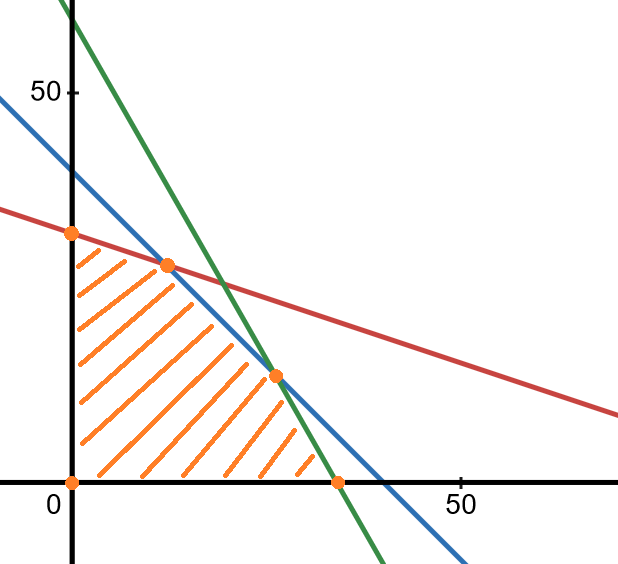
\includegraphics[width=0.3\linewidth]{./img/lp_brewery_problem.png}
        \caption{Feasible regions and vertexes of the polyhedron}
    \end{figure}

    In standard form, it becomes:
    \begin{center}
        \begin{tabular}{lccccccccccc}
            $\max$ & $13A$ & $+$ & $23B$ \\
            subj. to & $5A$ & $+$ & $15B$ & $+$ & $S_C$ & & & & & $=$ & 480 \\
                & $4A$ & $+$ & $4B$ & & & $+$ & $S_H$ & & & $=$ & 160 \\
                & $35A$ & $+$ & $20B$ & & & & & $+$ & $S_M$ & $=$ & 1190 \\
                & $A$ & , & $B$ & , & $S_C$ & , & $S_H$ & , & $S_M$ & $\geq$ & 0 \\
        \end{tabular}
    \end{center}
\end{example}



\section{Simplex algorithm}

Algorithm that starts from an extreme point of the polyhedron and iteratively moves to a neighboring vertex as long as the objective function does not decrease.


\subsection{Basis}

\begin{description}
    \item[Basis] \marginnote{Basis}
        Given an LP problem $\mathcal{P}$ in standard form with $m$ constraints and $n$ variables (note: in standard form, it holds that $m \leq n$) and
        its constraint matrix $\matr{A} \in \mathbb{R}^{m \times n}$,
        a (ordered) basis $\calB = \{ x_{i_1}, \dots, x_{i_m} \}$ is a subset of $m$ of the $n$ variables such that 
        the columns $\matr{A}_{i_1}, \dots, \matr{A}_{i_m}$ of $\matr{A}$ form a $m \times m$ invertible matrix $\matr{A}_\calB$.

        Variables in $\calB$ are basic variables while 
        $\calN = \{ x_1, \dots, x_n \} \smallsetminus \calB$ are non-basic variables.

        $\mathcal{P}$ can be rewritten by separating basic and non-basic variables:
        \[ 
            \max \{ \vec{c}_\calB \vec{x}_\calB  + \vec{c}_\calN\vec{x}_\calN \} \text{ subject to } 
                \matr{A}_\calB \vec{x}_\calB + \matr{A}_\calN \vec{x}_\calN = \vec{b} \,\land\, \vec{x}_\calB, \vec{x}_\calN \geq \nullvec 
        \]

    \item[Basic solution] \marginnote{Basic solution}
        By constraining $\vec{x}_\calN = \nullvec$, an LP problem becomes:
        \[ 
            \max \{ \vec{c}_\calB \vec{x}_\calB \} \text{ subject to } 
                \matr{A}_\calB \vec{x}_\calB = \vec{b} \,\land\, \vec{x}_\calB \geq \nullvec 
        \]
        As $\matr{A}_\calB$ is invertible by definition, it holds that:
        \[ 
            \vec{x}_\calB = \matr{A}_\calB^{-1} \vec{b} \hspace{2em}\text{ and }\hspace{2em} 
            \max \{ \vec{c}_\calB \vec{x}_\calB \} = \max \{ \vec{c}_\calB \matr{A}_\calB^{-1} \vec{b} \} 
        \]
        $\vec{x}_\calB$ is a basic solution for $\calB$.

    \item[Basic feasible solution (BFS)] \marginnote{Basic feasible solution (BFS)}
        Given a basic solution $\vec{x}_\calB$ for $\calB$,
        it is feasible iff:
        \[ \forall_{i=1}^m \vec{x}_{\calB_i} \geq 0 \]

        \begin{description}
            \item[Non-degenerate BFS] \marginnote{Non-degenerate BFS}
                A basic feasible solution is non-degenerate iff $\forall_{i=1}^m \vec{x}_{\calB_i} > 0$.
                \begin{remark}
                    A non-degenerate BFS is represented by a unique basis.
                \end{remark}
        \end{description}

        \begin{remark}
            The simplex algorithm iteratively moves through basic feasible solutions $\tilde{\vec{x}}_1, \tilde{\vec{x}}_2, \dots$
            such that $\vec{c}\tilde{\vec{x}}_k \geq \vec{c}\tilde{\vec{x}}_{k-1}$.
        \end{remark}
\end{description}


\subsection{Tableau}
\marginnote{Tableau}

Tabular representation to describe the steps of the simplex algorithm.
A variable $Z$ is introduced to represent the value of the objective function (which can be seen as a conversion of the objective function into a constraint).

The tableau of an LP problem in standard form is divided into three sections:
\begin{enumerate}
    \item Objective function, where the coefficients of the variables are called reduced costs\marginnote{Reduced costs}.
    \item Equality constraints.
    \item Variable constraints.
\end{enumerate}

\begin{example}[Brewery problem]
    In standard form, the brewery problem is defined as:
    \begin{center}
        \begin{tabular}{lccccccccccc}
            $\max$ & $13A$ & $+$ & $23B$ \\
            subj. to & $5A$ & $+$ & $15B$ & $+$ & $S_C$ & & & & & $=$ & 480 \\
                & $4A$ & $+$ & $4B$ & & & $+$ & $S_H$ & & & $=$ & 160 \\
                & $35A$ & $+$ & $20B$ & & & & & $+$ & $S_M$ & $=$ & 1190 \\
                & $A$ & , & $B$ & , & $S_C$ & , & $S_H$ & , & $S_M$ & $\geq$ & 0 \\
        \end{tabular}
    \end{center}

    As a tableau, assuming an initial basis $\calB = \{ S_C, S_H, S_M \}$, the problem is represented as:
    \begin{center}
        \begin{tabular}{cccccccccccccc}
            \toprule
            $13A$ & $+$ & $23B$ & & & & & & & $-$ & $Z$ & $=$ & 0 \\
            \midrule
            $5A$ & $+$ & $15B$ & $+$ & $S_C$ & & & & & & & $=$ & 480 \\
            $4A$ & $+$ & $4B$ & & & $+$ & $S_H$ & & & & & $=$ & 160 \\
            $35A$ & $+$ & $20B$ & & & & & $+$ & $S_M$ & & & $=$ & 1190 \\
            \midrule
            $A$ & , & $B$ & , & $S_C$ & , & $S_H$ & , & $S_M$ & & & $\geq$ & 0 \\
            \bottomrule
        \end{tabular}
    \end{center}
    The reduced costs are $\{ 13, 23, 0, 0, 0 \}$.
\end{example}


\subsection{Pivoting}

Given a basis $\calB$, it is possible to insert a new variable $x^\text{in} \notin \calB$ into it and remove an old one $x^\text{out} \in \calB$ 
to increase (or leave unchanged) the objective function:

\begin{descriptionlist}
    \item[Entering variable] \marginnote{Entering variable}
        $x^\text{in}$ should be the variable in $\calN$ with the highest improvement on the objective function.

    \item[Leaving variable] \marginnote{Leaving variable}
        $x^\text{out}$ should be chosen to ensure that the new basis $\calB' = \calB \cup \{ x^\text{in} \} \smallsetminus \{ x^\text{out} \}$
        is still a feasible basis.

        \begin{description}
            \item[Minimum ratio rule] \marginnote{Minimum ratio rule}
                For each constraint $i$ (i.e. $i$-th row of the system $\matr{A}\vec{x} = \vec{b}$), it is possible to compute the ratio:
                \[ \frac{\vec{b}_i}{\vec{\alpha}_i^\text{in}} \]
                where:
                \begin{itemize}
                    \item $\vec{\alpha}_i^\text{in}$ is the coefficient associated to the entering variable $x^\text{in}$ in the $i$-th constraint.
                    \item $\vec{b}_i$ is the known term of the $i$-th constraint.
                \end{itemize}

                The index $i$ of the leaving variable $x^\text{out} = \calB_i$ is determined as: 
                \[ \arg\min_i \frac{\vec{b}_i}{\vec{\alpha}_i^\text{in}} \]
        \end{description}
\end{descriptionlist}

Once $x^\text{in}$ and $x^\text{out} = \calB_i$ has been determined, 
$x^\text{in}$ is isolated in the equation of the $i$-th constraint and it is substituted in all the others.

\begin{example}[Brewery problem]
    The initial tableau of the brewery problem with $\calB = \{ S_C, S_H, S_M \}$ and $\calN = \{ A, B \}$ is:
    \begin{center}
        \begin{tabular}{cccccccccccccc}
            \toprule
            $13A$ & $+$ & $23B$ & & & & & & & $-$ & $Z$ & $=$ & 0 \\
            \midrule
            $5A$ & $+$ & $15B$ & $+$ & $S_C$ & & & & & & & $=$ & 480 \\
            $4A$ & $+$ & $4B$ & & & $+$ & $S_H$ & & & & & $=$ & 160 \\
            $35A$ & $+$ & $20B$ & & & & & $+$ & $S_M$ & & & $=$ & 1190 \\
            \midrule
            $A$ & , & $B$ & , & $S_C$ & , & $S_H$ & , & $S_M$ & & & $\geq$ & 0 \\
            \bottomrule
        \end{tabular}
    \end{center}

    \begin{enumerate}
        \item 
            It can be easily seen that $x^\text{in} = B$ should be the entering variable.
        
            For the leaving variable, the ratios are:
            \[ \arg\min \left\{ \frac{480}{15}, \frac{160}{4}, \frac{1190}{20} \right\} = \arg\min \left\{ 32, 40, 59.5 \right\} = 1 \]
            Therefore, the leaving variable is $x^\text{out} = \calB_1 = S_C$.
        
            We now isolate $B$ from the first constraint:
            \[ 
                \begin{split}
                    5A + 15B + S_C = 480 &\iff \frac{1}{3}A + B + \frac{1}{15}S_C = 32 \\
                        &\iff B = 32 - \frac{1}{3}A - \frac{1}{15}S_C \\
                \end{split}
            \]

            The tableau with $\calB' = \{ B, S_H, S_M \}$ and $\calN' = \{ A, S_C \}$ is updated as:
            \begin{center}
                \begin{tabular}{cccccccccccccc}
                    \toprule
                    $\frac{16}{3}A$ & & & $-$ & $\frac{23}{15}S_C$ & & & & & $-$ & $Z$ & $=$ & $-736$ \\
                    \midrule
                    $\frac{1}{3}A$ & $+$ & $B$ & $+$ & $\frac{1}{15}S_C$ & & & & & & & $=$ & $32$ \\
                    $\frac{8}{3}A$ & & & $-$ & $\frac{4}{15}S_C$ & $+$ & $S_H$ & & & & & $=$ & $32$ \\
                    $\frac{85}{3}A$ & & & $-$ & $\frac{4}{3}S_C$ & & & $+$ & $S_M$ & & & $=$ & $550$ \\
                    \midrule
                    $A$ & , & $B$ & , & $S_C$ & , & $S_H$ & , & $S_M$ & & & $\geq$ & 0 \\
                    \bottomrule
                \end{tabular}
            \end{center}

        \item 
            Now, $x^\text{in} = A$ is the variable that increases the objective function the most.

            For the leaving variable, the ratios are:
            \[ \arg\min \left\{ \frac{32}{1/3}, \frac{32}{8/3}, \frac{550}{85/3} \right\} = 2 \]
            Therefore, the leaving variable is $x^\text{out} = \calB'_2 = S_H$.

            $A$ isolated in the second constraint brings to:
            \[ 
                \begin{split}
                    A = \frac{3}{8} (32 + \frac{4}{15}S_C - S_H) \,\iff\, A = 12 + \frac{1}{10}S_C - \frac{3}{8}S_H
                \end{split}    
            \]

            The tableau with $\calB'' = \{ A, B, S_M \}$ and $\calN'' = \{ S_C, S_H \}$ is updated as:
            \begin{center}
                \begin{tabular}{cccccccccccccc}
                    \toprule
                     & & & $-$ & $S_C$ & $-$ & $2S_H$ & & & $-$ & $Z$ & $=$ & $-800$ \\
                    \midrule
                    & & $B$ & $+$ & $\frac{1}{10}S_C$ & $+$ & $\frac{1}{8}S_H$ & & & & & $=$ & $28$ \\
                    $A$ & & & $-$ & $\frac{1}{10}S_C$ & $+$ & $\frac{3}{8}S_H$ & & & & & $=$ & $12$ \\
                    & & & $-$ & $\frac{25}{6}S_C$ & $-$ & $\frac{85}{8}S_H$ & $+$ & $S_M$ & & & $=$ & $210$ \\
                    \midrule
                    $A$ & , & $B$ & , & $S_C$ & , & $S_H$ & , & $S_M$ & & & $\geq$ & 0 \\
                    \bottomrule
                \end{tabular}
            \end{center}

            We cannot continue anymore as the reduced costs $\{ 0, 0, -1, -2, 0 \}$ are $\leq 0$ (i.e. cannot improve the objective function anymore).
    \end{enumerate}
\end{example}


\subsection{Optimality}
\marginnote{Optimality}

When any substitution worsens the objective function, the current assignment is optimal.
In the tableau, this happens when all the reduced costs are $\leq 0$.

\begin{remark}
    For any optimal solution, there is at least a basis such that the reduced costs are $\leq 0$.
    Therefore, this is a sufficient condition.
\end{remark}

\begin{remark}
    The fact that reduced costs are $\leq 0$ is not a necessary condition.
\end{remark}

\begin{example}[Brewery problem]
    The tableau at the last iteration, with $\calB'' = \{ A, B, S_M \}$ and $\calN'' = \{ S_C, S_H \}$, is the following:
    \begin{center}
        \begin{tabular}{cccccccccccccc}
            \toprule
             & & & $-$ & $S_C$ & $-$ & $2S_H$ & & & $-$ & $Z$ & $=$ & $-800$ \\
            \midrule
            & & $B$ & $+$ & $\frac{1}{10}S_C$ & $+$ & $\frac{1}{8}S_H$ & & & & & $=$ & $28$ \\
            $A$ & & & $-$ & $\frac{1}{10}S_C$ & $+$ & $\frac{3}{8}S_H$ & & & & & $=$ & $12$ \\
            & & & $-$ & $\frac{25}{6}S_C$ & $-$ & $\frac{85}{8}S_H$ & $+$ & $S_M$ & & & $=$ & $210$ \\
            \midrule
            $A$ & , & $B$ & , & $S_C$ & , & $S_H$ & , & $S_M$ & & & $\geq$ & 0 \\
            \bottomrule
        \end{tabular}
    \end{center}

    All reduced costs are $\leq 0$ and an optimal solution has been reached:
    \begin{itemize}
        \item $S_C = 0$ and $S_H = 0$ (variables in $\calN''$).
        \item $A = 12$, $B = 28$ and $S_M = 210$ (variables in $\calB''$. Obtained by isolating them in the constraints).
        \item $- S_C - 2S_H - Z = -800 \iff Z = 800 - S_C - 2S_H \iff Z = 800$ (objective function).
    \end{itemize}
\end{example}

\begin{remark}
    The points in the feasible region of a problem $\mathcal{P}$ are:
    \[ \mathcal{F}_\mathcal{P} = \{ \vec{x} \in \mathbb{R}^n \mid \matr{A}\vec{x} \leq \vec{b} \land \vec{x} \geq \nullvec \} \]
\end{remark}

\begin{description}
    \item[Optimal region] \marginnote{Optimal region}
        For an LP problem $\mathcal{P}$, its set of solutions is defined as:
        \[ \mathcal{O}_\mathcal{P} = \{ x^* \in \mathcal{F}_\mathcal{P} \mid \forall \vec{x} \in \mathcal{F}_\mathcal{P}: \vec{c}\vec{x}^* \geq \vec{c}\vec{x} \} \]

        Trivially, it holds that $\mathcal{O}_\mathcal{P} \subseteq \mathcal{F}_\mathcal{P}$ and 
        $\mathcal{F}_\mathcal{P} = \varnothing \Rightarrow \mathcal{O}_\mathcal{P} = \varnothing$.

        \begin{theorem}
            If $\mathcal{O}_\mathcal{P}$ is finite, then $\vert \mathcal{O}_\mathcal{P} \vert = 1$ 
            (therefore, if $\vert \mathcal{O}_\mathcal{P} \vert > 1$, then $\mathcal{O}_\mathcal{P}$ is infinite).
        \end{theorem}
\end{description}

\begin{description}
    \item[Unbounded problem] \marginnote{Unbounded problem} 
        An LP problem $\mathcal{P}$ is unbounded if it does not have an optimal solution (i.e. $\mathcal{F}_\mathcal{P}$ is an unbounded polyhedron).

        With the tableau formulation, if a column has reduced cost $> 0$ and all the constraint coefficients are $\leq 0$, then the problem is unbounded.

        \begin{example}
            Given the following tableau:
            \begin{center}
                \begin{tabular}{cccccccccccc}
                    \toprule
                    & $x$ & $-$ & $y$ & & & & & $-$ & $Z$ & $=$ & $-1$ \\
                    \midrule
                    $-$ & $x$ & $-$ & $y$ & $+$ & $S_1$ & & & & & $=$ & $0$ \\
                    $-$ & $2x$ & $-$ & $y$ & & & $+$ & $S_2$ & & & $=$ & $1$ \\
                    \midrule
                    & $x$ & , & $y$ & , & $S_1$ & , & $S_2$ & & & $\geq$ & 0 \\
                    \bottomrule
                \end{tabular}
            \end{center}
            The unboundedness of the problem can be detected from the first column.

            \begin{figure}[H]
                \centering
                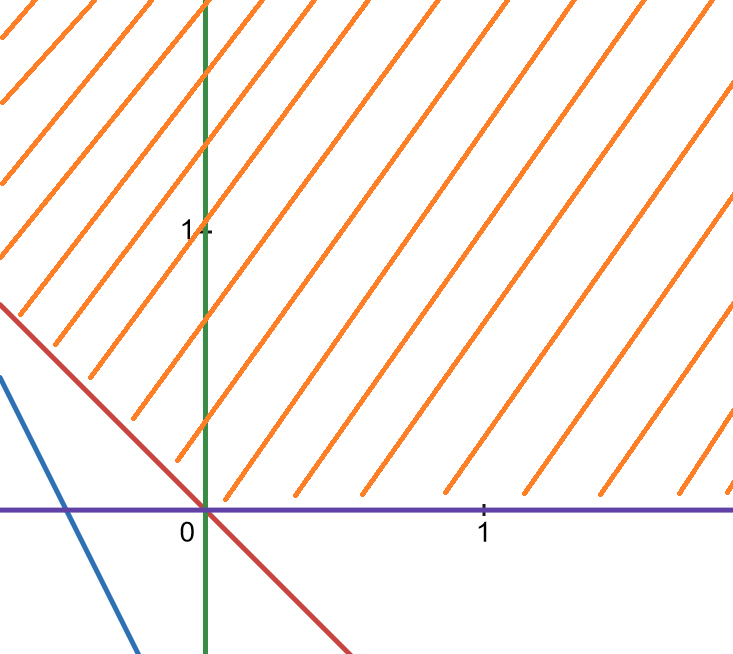
\includegraphics[width=0.3\linewidth]{./img/lp_unbounded.png}
            \end{figure}
    \end{example}
\end{description}


\subsection{Algorithm}

Given an LP problem $\mathcal{P}$ in standard form, the steps of the simplex algorithm are:
\begin{enumerate}
    \item Set $k=0$, find a feasible basis $\calB_k$ and reformulate $\mathcal{P}$ according to it.
    \item If the basis feasible solution is optimal, return.
    \item If $\mathcal{P}$ is unbounded, return.
    \item Select an entering variable $x^\text{in}$.
    \item Select a leaving variable $x^\text{out}$.
    \item Let $\calB_{k+1} = \calB_k \cup \{ x^\text{in} \} \smallsetminus \{ x^\text{out} \}$ and reformulate $\mathcal{P}$ according to the new basis.
    \item Set $k = k + 1$ and go to Point 2.
\end{enumerate}

\begin{description}
    \item[Properties] \phantom{}
        \begin{itemize}
            \item If all basis feasible solutions are non-degenerate, the simplex algorithm always terminates (as the solution is always strictly improving).
            \item In the general case, the algorithm might stall by ending up in a loop.
            \item The worst-case time complexity is $O(2^n)$. The average case is polynomial.
        \end{itemize}
\end{description}

\begin{remark}
    If the problem has lots of vertexes, the interior point method (polynomial complexity) or approximation algorithms should be preferred.
\end{remark}


\subsection{Two-phase method}
\marginnote{Two-phase method}

Method that solves an LP problem by first finding an initial feasible basis $\calB_0$ and determining if the LP problem is unsatisfiable.

Given an LP problem $\mathcal{P}$ ($\max\{ \vec{cx} \} \text{ subject to } \matr{A}\vec{x} = \vec{b}$ with $m$ constraints and $n$ variables), 
the two-phase method works as follows:
\begin{descriptionlist}
    \item[Phase 1] 
        Define a new artificial problem $\mathcal{P}'$ from $\mathcal{P}$ with new variables $s_1, \dots, s_m$ as follows:
        \[
            \begin{split}
                \max\left\{ -\sum_{i=1}^{m} s_i \right\} \text{ subject to } 
                    &\sum_{j=1}^{n} a_{i,j} x_j + s_i = b_i \text{ for } i \in \{ k \in \{ 1, \dots, m \} \mid b_k \geq 0 \} \,\land \\
                    &\sum_{j=1}^{n} a_{i,j} x_j - s_i = b_i \text{ for } i \in \{ k \in \{ 1, \dots, m \} \mid b_k < 0 \} \,\land \\
                    & s_i, x_j \geq 0
            \end{split}
        \]

        \begin{remark}
            It holds that $-\sum_{i=1}^{m} s_i \leq 0$ and 
            $\calB' = \{ s_1, \dots, s_m \}$ is always a feasible basis corresponding to the basis feasible solution $x_j = 0$, $s_i = \vert b_i \vert$
        \end{remark}

        The problem $\mathcal{P}'$ with basis $\calB'$ can be solved through the simplex method.

        \begin{theorem}
            Let $\mathcal{F}_\mathcal{P}$ be the feasible region of $\mathcal{P}$. It holds that:
            \[ \mathcal{F}_\mathcal{P} \neq \varnothing \,\iff\, \sum_{i=1}^{m} s_i = 0 \]

            In other words:
            \begin{itemize}
                \item If the optimal solution of $\mathcal{P}'$ is  $< 0$, then $\mathcal{P}$ is unsatisfiable.
                \item Otherwise, the basis $\calB_{\mathcal{P}'}$ corresponding to the optimal solution of $\mathcal{P}'$ 
                    can be used as the initial basis of $\mathcal{P}$, after removing the variables $s_i$.
            \end{itemize}
        \end{theorem}

    \item[Phase 2] 
        Solve $\mathcal{P}$ through the simplex algorithm using as initial basis $\calB_{\mathcal{P}'}$.
\end{descriptionlist}


\subsection{Duality}

\begin{description}
    \item[Dual problem]
        Given the primal problem $P$ defined as: 
        \[ P: \max \{\vec{cx}\} \text{ subject to } \matr{A}\vec{x} = \vec{b} \land \vec{x} \geq \nullvec \]
        with $\vec{b} \in \mathbb{R}^m$, $\vec{x} \in \mathbb{R}^n$, $\matr{A} \in \mathbb{R}^{m \times n}$,
        its dual problem $\mathcal{D}(P)$ is defined as:
        \[ \mathcal{D}(P): \min\{\vec{by}\} \text{ subject to } \matr{A}^T\vec{y} \geq \vec{c} \land \vec{y} \geq \nullvec \]
        where:
        \begin{itemize}
            \item $\vec{y} \in \mathbb{R}^m$ has a variable $\vec{y}_i$ for each constraint $\sum_{j=1}^{n} \matr{A}_{i,j} \vec{x}_j = \vec{b}_i$ of $P$,
            \item $\sum_{i=1}^{m} \matr{A}_{j, i} \vec{y}_i \geq \vec{c}_j$ is a new constraint defined for each variable $\vec{x}_j$ of $P$.
        \end{itemize} 

        \begin{remark}
            The constraint $\vec{y} \geq \nullvec$ comes out naturally from the conversion from primal to dual.
            Therefore, it is not strictly necessary to explicitly put it.
        \end{remark}

        \begin{example}
            Given the primal problem:
            \begin{center}
                \begin{tabular}{lccccccccccc}
                    \toprule
                    $\max$ & $1x_1$ & $+$ & $1x_2$ & $+$ & \color{lightgray}$0x_3$ & $+$ & \color{lightgray}$0x_4$ & $+$ & \color{lightgray}$0x_5$ \\
                    \midrule
                    subj. to & $3x_1$ & $+$ & $2x_2$ & $+$ & $1x_3$ & $+$ & \color{lightgray}$0x_4$ & $+$ & \color{lightgray}$0x_5$ & $=$ & 5 \\
                             & $4x_1$ & $+$ & $5x_2$ & $+$ & \color{lightgray}$0x_3$ & $+$ & $1x_4$ & $+$ & \color{lightgray}$0x_5$ & $=$ & 4 \\
                             & \color{lightgray}$0x_1$ & $+$ & $1x_2$ & $+$ & \color{lightgray}$0x_3$ & $+$ & \color{lightgray}$0x_4$ & $+$ & $1x_5$ & $=$ & 2 \\
                    \midrule
                            & $x_1$ & , & $x_2$ & , & $x_3$ & , & $x_4$ & , & $x_5$ & $\geq$ & 0 \\
                    \bottomrule
                \end{tabular}
            \end{center}

            Its dual is:
            \begin{center}
                \begin{tabular}{lccccccc}
                    \toprule
                    $\min$ & $5y_1$ & $+$ & $4y_2$ & $+$ & $2y_3$ \\
                    \midrule
                    subj. to & $3y_1$ & $+$ & $4y_2$ & $+$ & \color{lightgray}$0y_3$ & $\geq$ & 1 \\
                             & $2y_1$ & $+$ & $5y_2$ & $+$ & $1y_3$ & $\geq$ & 1 \\
                             & $1y_1$ & $+$ & \color{lightgray}$0y_2$ & $+$ & \color{lightgray}$0y_3$ & $\geq$ & 0 \\
                             & \color{lightgray}$0y_1$ & $+$ & $1y_2$ & $+$ & \color{lightgray}$0y_3$ & $\geq$ & 0 \\
                             & \color{lightgray}$0y_1$ & $+$ & \color{lightgray}$0y_2$ & $+$ & $1y_3$ & $\geq$ & 0 \\
                    \bottomrule
                \end{tabular}
            \end{center}
        \end{example}
\end{description}

\begin{theorem}
    For any primal problem $P$, it holds that $\mathcal{D}(\mathcal{D}(P)) = P$.
\end{theorem}

\begin{theorem}[Weak duality] \marginnote{Weak duality}
    The cost of any feasible solution of the primal $P$ is less or equal than the cost of any solution of the dual $\mathcal{D}(P)$:
    \[ \forall \vec{x} \in \mathcal{F}_{P}, \forall \vec{y} \in \mathcal{F}_{\mathcal{D}(P)}: \vec{cx} \leq \vec{by} \]

    In other words, $\vec{by}$ is an upper bound for $P$ and $\vec{cx}$ is a lower bound for $\mathcal{D}(P)$.

    \begin{corollary}
        If $P$ is unbounded, then $\mathcal{D}(P)$ is unfeasible:
        \[ \mathcal{F}_{P} \neq \varnothing \land \mathcal{O}_{P} = \varnothing \,\,\Rightarrow\,\, \mathcal{F}_{\mathcal{D}(P)} = \varnothing \]
    \end{corollary}

    \begin{corollary}
        If $\mathcal{D}(P)$ is unbounded, then $P$ is unfeasible:
        \[ \mathcal{F}_{\mathcal{D}(P)} \neq \varnothing \land \mathcal{O}_{\mathcal{D}(P)} = \varnothing \,\,\Rightarrow\,\, \mathcal{F}_{P} = \varnothing \]
    \end{corollary}
\end{theorem}

\begin{theorem}[Strong duality] \marginnote{Strong duality}
    If the primal and the dual are feasible, then they have the same optimal values:
    \[ 
        \Big( \mathcal{F}_{P} \neq \varnothing \land \mathcal{F}_{\mathcal{D}(P)} \neq \varnothing \Big) \Rightarrow 
        \Big( \forall \vec{x}^* \in \mathcal{O}_P, \forall \vec{y}^* \in \mathcal{O}_{\mathcal{D}(P)}: \vec{cx}^* = \vec{by}^* \Big)
    \]
\end{theorem}

\begin{description}
    \item[Dual simplex] \marginnote{Dual simplex}
        Move from optimal basis (which can be unfeasible) to feasible basis, while preserving optimality.

        \begin{remark}
            The traditional primal simplex moves from feasible to optimal basis, while preserving feasibility.
        \end{remark}

    \item[Properties]
        \phantom{}
        \begin{itemize}
            \item Duality makes the time complexity of finding a feasible or optimal solution the same.
            \item The dual allows to prove the unfeasibility of the primal.
            \item Primal and dual provide a bounding of the objective function.
        \end{itemize}
\end{description}


\subsection{Sensitive analysis}
\marginnote{Sensitive analysis}

Study how the optimal solution of a problem $P$ is affected if $P$ is perturbed.

Given a problem $P$ with optimal solution $\vec{x}^*$, a perturbed problem $\bar{P}$ can be obtained by altering:
\begin{descriptionlist}
    \item[Known terms] 
        Change of form: 
        \[ \vec{b} \leadsto \bar{\vec{b}} = \vec{b} + \Delta \vec{b} \]
        This can affect the feasibility and optimality of $\vec{x}^*$.

        \begin{remark}
            Changing the known terms of $P$ changes the objective function of $\mathcal{D}(P)$.
        \end{remark}

    \item[Objective function coefficients] 
        Change of form: 
        \[ \vec{c} \leadsto \bar{\vec{c}} = \vec{c} + \Delta \vec{c} \]
        This can affect the optimality of $\vec{x}^*$.
    
    \item[Constraint coefficients] 
        Change of form: 
        \[ \matr{A} \leadsto \bar{\matr{A}} = \matr{A} + \Delta \matr{A} \]
        \begin{itemize}
            \item If the change involves a variable $\vec{x}^*_j = 0$, then feasibility is not changed but optimality can be affected.
            \item If the change involves a variable $\vec{x}^*_j \neq 0$, the problem needs to be re-solved.
        \end{itemize}
\end{descriptionlist}



\section{(Mixed) integer linear programming}

\begin{description}
    \item[Integer linear programming (ILP)] \marginnote{Integer linear programming (ILP)}
        Linear programming problem where variables are all integers:
        \[ 
            \begin{split}
                \max \sum_{j=1}^{n} c_j x_j \text{ subject to } &\sum_{j=1}^{n} a_{i,j} x_j = b_i \,\,\text{ for } 1 \leq i \leq m \,\,\land \\
                    & x_j \geq 0 \land x_j \in \mathbb{Z} \,\,\text{ for } 1 \leq j \leq n
            \end{split}
        \]

    \item[Mixed-integer linear programming (MILP)] \marginnote{Mixed-integer programming (MILP)}
        Linear programming problem with $n$ variables where $k < n$ variables are integers.
\end{description}

\begin{theorem}
    Finding a feasible solution of a mixed-integer linear programming problem is NP-complete.

    \begin{proof}
        \phantom{}
        \begin{descriptionlist}
            \item[MILP in NP)] 
                A certificate contains an assignment of the variables. It is sufficient to check if all constraints are satisfied.
                Both steps are polynomial.
            \item[MILP is NP-hard)] 
                Any SAT problem can be poly-reduced to MILP.
        \end{descriptionlist}
    \end{proof}
\end{theorem}

\begin{remark}
    Due to its NP-completeness, MILP problems can be solved by:
    \begin{descriptionlist}
        \item[Exact algorithms] Guarantee optimal solution with exponential time complexity.
        \item[Approximate algorithms] Guarantee polynomial time complexity but might provide sub-optimal solutions with an approximation factor $\rho$.
        \item[Heuristic algorithms] Empirically find a good solution in a reasonable time (no theoretical guarantees).
    \end{descriptionlist}
\end{remark}


\subsection{Linear relaxation}
\marginnote{Linear relaxation}

Given a MILP problem $P$, its linear relaxation $\mathcal{L}(P)$ removes the constraints $x_j \in \mathbb{Z}$.
However, solving $\mathcal{L}(P)$ as an LP problem and rounding the solution does not guarantee feasibility or optimality.

\begin{theorem}
    It holds that $\mathcal{F}_{\mathcal{L}(P)} = \varnothing \Rightarrow \mathcal{F}_P = \varnothing$.

    Therefore, the linear relaxation of a MILP problem can be used to verify unsatisfiability.
\end{theorem}

\begin{remark}
    If $\mathcal{F}_{\mathcal{L}(P)}$ is unbounded, then $P$ can either be bounded, unbounded or unsatisfiable.
\end{remark}



\subsection{Branch and bound}